\documentclass[a4paper,11pt]{refart}
\usepackage{listingsutf8}
\usepackage[utf8]{inputenc}
\usepackage[T1]{fontenc} % LY1 also works
\usepackage{tikz}
\usetikzlibrary{shapes,arrows}
%% Font settings suggested by fbb documentatio
\usepackage{float} 
\usepackage{listings}
\usepackage{microtype}
\usepackage{graphicx}
\usepackage{enumitem}
\setlist{leftmargin=*}
\lstset{basicstyle=\ttfamily,frame=single,xleftmargin=1em,xrightmargin=1em}
\usepackage[os=win]{menukeys}
\renewmenumacro{\keys}[+]{shadowedroundedkeys}
\usepackage{framed}
\usepackage{etoolbox}
\AtBeginEnvironment{leftbar}{\sffamily\small}
\usepackage[T1]{fontenc}
\usepackage{lmodern}
\usepackage{hyperref}
\usepackage{multirow}                                               
\usepackage{multicol}                                               
\usepackage{longtable}
\usepackage{amsmath}
\usepackage{dcolumn}
\usepackage{booktabs}
\usepackage{makecell}

\renewcommand\theadalign{bc}
\renewcommand\theadfont{\bfseries}
\renewcommand\theadgape{\Gape[4pt]}
\renewcommand\cellgape{\Gape[4pt]}


\renewcommand\abstractname{Introduction}
\def\CS#1{\texttt{\textbackslash#1}}

\usepackage[most]{tcolorbox}
\newtcblisting{commandshell}{colback=black,colupper=green,colframe=black!75!black,
	listing only,listing options={style=tcblatex,language=sh},
	every listing line={\textcolor{red}{\small\ttfamily\bfseries computer@user:\$ }}}

\usepackage[most]{tcolorbox}
\newtcblisting{shell}{colback=black,colupper=green,colframe=black!75!black,
	listing only,listing options={style=tcblatex,language=sh},
	every listing line={\textcolor{red}{\small\ttfamily\bfseries  }}}


\title{PRIMoRDiA 1.0v User Guide}
\author{Igor Barden Grillo \\(\url{PRIMoRDiA.software@gmail.com} )\\\url{github.com/igorChem}}
	
\begin{document}
\maketitle

\begin{abstract}
PRIMoRDiA ( \textbf{PRI}MoRDiA \textbf{M}acromolecular \textbf{R}eactivity \textbf{D}escriptors \textbf{A}ccess ) ia a shared memory parallel software written in C++ for post electronic structure calculations, that efficiently read output files from most used quantum mechanics packages, storing molecular information and processing it to generate several descriptors to evaluate the global and local reactivity of molecular systems. PRIMoRDiA supports the main reactivity descriptors of the Conceptual Density Functional Theory, the most famous and used reactivity theory, which work from response variables of the electronic structure of the molecules, as also other electrostatics properties.

This guide resumes: 
\begin{enumerate}
	\item Download and installation
	\item Theoretical review
	\item General usage
	\item Specific options
	\item Information needed from the quantum mechanical packages output ( how to build their input files )
	\item Input format and reactivity descriptors options.
	\item List of generated files and descriptors.
	\item How to work with the generated scripts for usage of graphical packages.
	\item All purpose tutorials.
\end{enumerate}

\end{abstract}
\newpage
\tableofcontents
\newpage

\section{Download and Installation}

Our Github repository, that contains the executable, this userguide and the test set, can be downloaded or cloned at https://github.com/igorChem/PRIMoRDiA1.0v.git. If you download you will have to extract the zip file. To clone the repository run the following command

\hspace*{-\leftmarginwidth}
\begin{minipage}{\fullwidth}
	\begin{commandshell}git clone https://github.com/igorChem/PRIMoRDiA1.0v.git\end{commandshell}
\end{minipage}

The executable, file named "PRIMoRDiA\_1.0v\_LINUX64", is compiled for linux machines with x86\_64 architecture and ready to use in such configurations. For ease use, the executable can be put in the path of your system with following command

\hspace*{-\leftmarginwidth}
\begin{minipage}{\fullwidth}
	\begin{commandshell}echo "alias primordia='/path/to/executable/PRIMoRDiA\_1.0v\_LINUX64'" >> ~/.bashrc
source ~/.bashrc\end{commandshell}
\end{minipage}

For avoid run problems and maximum performance, the system must have the amount of RAM at least equal to the files provided for analysis. This is relevant when dealing with macromolecules containing five thousand atoms or more. 



\section{Reactivity Descriptors}

Reactivity Descriptors (RD) are convenient theoretical quantities that summarize the reactive behavior of a molecular system or its atoms/different regions. The most successful and employed RD are from the Conceptual Density Functional Theory, that provided mathematical definitions of already used chemical concepts. This definitions are drawn from the fundamental differential equation of the DFT \autoref{eq.1}, and its Taylor series expansions, taking the energy and electron density derivatives with respect the number of electrons, and its Maxwell relations with other functional derivatives, assigning to it an reactive behavior for the system\cite{parr1978elect}. 

\begin{equation}
dE = \mu dN + \int \rho(r) d \nu (r) dr
\label{eq.1}
\end{equation}

The descriptors can be firstly separated by global, a number that represent all molecular system, and local quantity that is function of position. All global quantities that are outputted by PRIMoRDiA are listed in \autoref{tab1}, with its definition in CDFT and how the calculation occurs for each method available, Frozen Orbital Approximation (FOA) and Finite Differences (FD), that is the second possible way to categorize the RD. The third way to classify the access of these quantities is through the representation type, which is reserved only for the local RD, that can be represented by values at each point of a three dimensional grid or by a list of values, assigning the reactivity for each atomic center in the molecular system. The former representation type is called Condensed to atoms, often shortened in the literature as only condensed.    

\tikzstyle{block} = [rectangle, draw, fill=cyan!20, 
text width=5em, text centered, rounded corners, minimum height=4em]
\tikzstyle{decision} = [diamond, draw, fill=yellow!20, 
text width=4.5em, text badly centered, node distance=3cm, inner sep=0pt]
\tikzstyle{line} = [draw, -latex']

\begin{figure}[H]
	\centering
\begin{tikzpicture}[node distance = 2.5cm, auto]
\node [block] (init) {CDFT Descriptors};
\node [decision, below of=init] (typerd) {RD scope};
\node [block, right of=typerd] (local) {Local};
\node [block, left of=typerd] (global) {Global};
\node [decision, right of=local] (rep) {Display};
\node [block, above of=rep] (cond) {Condensed};
\node [block, below of=rep] (vol) {3D Grid};
\node [decision, below of=typerd] (method) {Method};
\node [block, right of=method] (foa) {FOA};
\node [block, left of=method] (fd) {FD};
\path [line] (init) -- (typerd); 
\path [line] (typerd) -- (local); 
\path [line] (typerd) -- (global); 
\path [line] (global) -- (method);
\path [line] (local) -- (method);
\path [line] (local) -- (rep);
\path [line] (method) -- (foa);
\path [line] (method) -- (fd);
\path [line] (rep) -- (cond);
\path [line] (rep) -- (vol);
\end{tikzpicture}
\caption{Classification of the reactivity descriptors.} \label{fig:M1}
\end{figure}

%colocar imagem de um fluxograma representando os tipos de descritores e suas calssificações

The first CDFT RD that we can consider is the Electronic Chemical Potential (ECP), often represented by the Greek letter $\mu$, that is the first derivative of the electrons energy in respect of the number of electrons with external potential $\nu$ constant, and represents the electron escape tendency, i.e., the system likeness to donate electrons.
Pearson's Hard and Soft Acid and Base principles areanother chemical concept elevated to a more solid mathematical foundations by the CDFT development. 

The hardness $\eta$ is defined as either the second derivative of the energy with respect to the number of electrons or the derivative of ECP with respect to the number of electrons at a constant external potential; the softness $S$ is defined as its reciprocal. Other global RDs can be derived to provide charge transfer quantities, which can be used to characterize chemical reactions. The maximum number of electrons ($nMax$) that the system could receive from an ideal donor and the stabilization energy when these electrons are received, which is called the total electrophilicity ($\omega$), are examples of such global RDs \autoref{tab1}.

There are two current calculations methods for the CDFT RD which are supported by PRIMoRDiA. The first is the Finite Differences, that for the global RDs takes the electronic energy of different charged states to estimate the derivative values. This is necessary because the fact of the discontinuity in the number of electrons, i.e., there is no fractional number of electrons, at least in the conventional quantum mechanics treatments. The electronic energy assessment is done for the original charged states of the molecular system of interest, one negative charged (minimum one more electron). and one positive charged (minimum one electron less). All these three state calculations are performed for the same nuclei coordinates, conserving the requirement of constant external potential of the partial derivative.

The other calculation method is defined according to Koopmans Theorem[ref], which states that energies of the charge states can be approximated using Ionization Potential (IP) and Electron Affinity (EA). These quantities can be estimated using the energies of the Highest energy Occupied Molecular Orbital (HOMO) for IP and the Lowest energy Unoccupied Molecular Orbital (LUMO) for EA. In contrast with finite differences, the approximation from Koopmans theorem requires just a single point calculation to obtain the global RDs. In this approximation the relaxation energetic effect for the internal molecular orbital are not accounted because is considered negligible and thus called the Frozen Orbital Approximation. 

\hspace*{-\leftmarginwidth}
\begin{minipage}{\fullwidth}
	\begin{table}[H]
		\centering	
		\caption{Global Reactivity Descriptors calculated by the by PRIMoRDiA software}
		\begin{tabular}{c|c|c|c|c}
			\toprule
			Global RD & CDFT Definition & FOA & FD & Ref. \\
			\midrule
			IP & -  & $- E_{HOMO}$ & $E_{N-1}-E_{N}$  &  \\  \hline	
			EA & -  & $- E_{LUMO}$ & $E_{N}-E_{N+1}$ & \\ \hline	
			$\mu$  & $\left(\frac{\partial E}{\partial N} \right)_\nu$  & $\frac{E_{HOMO} + E_{LUMO}}{2}$ &$\frac{E_{N-1}-E_{N+1}}{2}$ & \cite{ribeiro2017atlas}\\ \hline			
			$\eta$  & $\left(\frac{\partial ^2  E}{\partial N ^2} \right)_\nu$ &$E_{LUMO} - E_{HOMO}$ &$E_{N-1}+E_{N+1}-2E_{N}$ & \cite{parr1983absolute}\\ \hline
			Softness($S$)  & $1/\eta$  & - & -  & \cite{parr1983absolute} \\ \hline
			$\omega$  & $\frac{\mu^2S}{2}$  &-  &-  & \cite{cedillo2012local} \\ \hline
			$nMax$  & $-\frac{\omega}{\eta} $ & - & - & \cite{cedillo2012local}  \\ 
			\bottomrule
		\end{tabular} 
	\label{tab1}	
	\end{table}	
\end{minipage}

Depending on the representation type, local RD are assigned to  points in the three dimensional space, called voxels (three-dimensional analogous of a pixel). This representations type can be accessed in graphical packages requiring surfaces with that hold the same values ( iso-surfaces ), or rendering several of its iso-surfaces, which is called volume. Commonly, a set of voxels forming a three dimensional grid covering all space where the atoms from molecular system are enclosed is written to a cube file. PRIMoRDiA generates this cube files for each local RD supported if was required in grid arguments a integer greater than zero. This files are formatted as standard GAUSSIAN cube files, where the main graphical packages can open. This local RD represented as scalar fields are functions of three-dimensional coordinate $r$. 

The Fukui indices are the first local RD in CDFT and its calculations are required for the great majority of others local RD. Which is also called the Fukui function, the derivative of electron density in respect to the number of electrons(\autoref{eq.2}), that also is extracted from the \autoref{eq.1}\cite{Parr1984}. The regions in the molecular system where the Fukui function values are at maximum is indicated where are the great propensity to the electron density to increase as the number of electrons vary.
   
\begin{equation}
f(r) = \left(\frac{\partial \rho(r)}{\partial N} \right)_\nu
\label{eq.2}
\end{equation}

The Fukui function characterizes intramolecular reactivity, which makes it useful for identifying the selectivity of a given electrophilic, nucleophilic or radical attack, each of which are represented by a given Fukui function. Fukui functions were initially developed to be calculated using FD in relation to the electron densities of charged states. With these descriptors, it is possible to say how the electron density will change when another system approaches and thus promote a change in the number of electrons. In other words, the system part where the descriptor is at its maximum is where the electron density will concentrate to form a new bond.

Due to the discontinuity of the electrons, the FD calculus method was the first used to estimate the derivative, set in \autoref{eq.2}. The chosen method caused to the derivative to be defined at two definitions, one at the right of the $ \lim_{N \to 0}$ and to the left.  The electrophilic attack susceptibility (EAS), which is the left Fukui function ($f^{-}$) , reveals the regions where an electrophilic species is most likely to form a bond; the same explanation applies for nucleophilic attack susceptibility (NAS), right Fukui function ($f^{-}$), and for radical attack susceptibility (RAS), zero point Fukui function ($f^{0}$). The FD uses the electrons densities of different charged states to calculate the Fukui function, for EAS the difference between electron density $\rho(r)$ obtained from the molecular system with original charge (N electrons) and the electron density from the molecular system with decreased number of electrons (N-1, at least)\autoref{eq.3}. 

\begin{equation}
f^{-}(r) = \rho(r)_{N} -\rho(r)_{N-1}
\label{eq.3}
\end{equation}

The electron density is calculated from the sum of $i$ occupied molecular orbitals $\phi(r)$ square module\autoref{eq.4}, and the molecular orbitals are obtained from the linear combination of the atomic orbitals $\chi$ \autoref{eq.5}. The atomic orbitals can be a catesian slater basis set\autoref{eq.6}, which is for instance the standard for the semiempirical methods in MOPAC.  

\begin{equation}
\rho(r) = \sum_{i}^{occ} |\phi(r)^2_i|
\label{eq.4} 
\end{equation}

\begin{equation}
\phi(r)_i = \sum_{i} c_i \chi(r)
\label{eq.5} 
\end{equation}

\begin{equation}
\chi(r)_{kmn} = Nx^k y^m z^n \exp(- \zeta r)
\label{eq.6} 
\end{equation}

For NAS, the right Fukui function $f^{+}(r)$, the FD method defines the derivative as the difference of electron density of the molecular system with an increased number of electrons (N+1, at least) and the original charged state (N) electron density. Often the difference in charge is one to approximate at maximum to the limit, but this can change when the system needs a greater perturbation to show the more reactivity regions through these functions. For the FD option in PRIMoRDiA is required to indicate the charge difference used to calculated the other charged states to normalize the resulted Fukui functions to one.  

\begin{equation}
f^{+}(r) = \rho(r)_{N+1} -\rho(r)_{N}
\label{eq.8}
\end{equation}

The RAS. or zero point Fukui function, is defined as the arithmetic average of the EAS and NAS\autoref{eq.9}, which brings the possible interpretation of this descriptor to be a averaged Fukui function. 

\begin{equation}
f^{0}(r) = \frac{\rho(r)_{N+1} -\rho (r)_{N-1}}{2}
\label{eq.9}
\end{equation}

A fourth Fukui function can be considered, the Dual Fukui or Dual Descriptor, that can indicate simultaneous the electrophilic and nucleophilc attack susceptibility regions. This descriptor is calculated as the difference between NAS and EAS\autoref{eq.10}, also mitigating the Fukui function values in regions that present both behaviors, which make it to be a net Fukui function as well. Also, is claimed that this descriptors brings less errors because the possible cancellation in the difference between left and right Fukui functions  \cite{martinez2015dual}. 

\begin{equation}
\Delta f^{\pm} = f^{+}(r) - f^{-}(r)
\label{eq.10}
\end{equation}

A FOA definition also exists for local RD that are derived from Fukui functions, based on the fact that a infinitesimal change in the number of electrons the inner molecular orbitals would have a irrelevant contribution to the electron density and thus for the Fukui function itself. In EAS case the left Fukui function is defined in ways of $M$ one-electron molecular orbitals \autoref{eq.11}, that is the electron density derivative in respect to the number od electrons from the limit  of $\delta$ decreasing of electrons tending to zero. The equations is divided in one part for the contribution of the HOMO and other ,that are neglected in the FOA, for the inner molecular orbitals. The EAS for FOA turns to be the density of only the HOMO\autoref{eq.12}. The same occurs for the NAS, but the LUMO (M+1) is included, and the HOMO join the sum of the inner orbitals that are neglected \autoref{eq.13}, and NAS finally defines as the density of LUMO \autoref{eq.14}.  For RAS, the definition often follows the ones that were cited earlier in the text, being the average of EAS and NAS, but also can be thought as the density of the Single Occupied Molecular Orbital (SOMO)[ref]\autoref{eq.15}.

\begin{equation}
f^{-}(r) = \lim_{\delta \to 0} \frac{\partial \rho_{M+\delta}(r)}{\partial N} = |\phi_{M}(r)|^2  +\sum_{i=1}^{M-1} \frac{\partial}{\partial N} |\phi_i(r)|^2
\label{eq.11}
\end{equation}

\begin{equation}
f^{-}(r) = |\phi_{HOMO}(r)|^2 
\label{eq.12}
\end{equation}

\begin{equation}
f^{+}(r) = \lim_{\delta \to 0^+} \frac{\partial \rho_{M+\delta}(r)}{\partial N}	 =  |\phi_{M+1}(r)|^2 		 + \sum_{i=1}^{M} \frac{\partial}{\partial N} |\phi_i(r)|^2
\label{eq.13}
\end{equation}

\begin{equation}
f^{+}(r) = |\phi_{LUMO}(r)|^2 
\label{eq.14}
\end{equation}

\begin{equation}
f^{0}(r) = |\phi_{SOMO}(r)|^2 
\label{eq.15}
\end{equation}

The other representation type used to these local RD is the condensed, as already cited, where the reactivity values are assigned to each atomic center in the molecule. The \autoref{eq.11} shows the generic condensation method for a Fukui function, where its values are integrated to each point $r$ in space that is considered to the $k_th$ atom enclose.  

\begin{equation}
f_k^{a} = \int_{\Omega k} f(r)^{a}_{k}dr
\label{eq.16}
\end{equation}

In the FD case, the condensation is done around the partial gross charge of each atom, obtained originally from the Mulliken's Population analysis. EAS is defined for the $K_{th}$ atom as the difference of the partial charge in neutral and in the positive charged system\autoref{eq.17}, and NAS as the difference from the partial charge of negatively charged and the state with original charge\autoref{eq.18}.

\begin{equation}
f^{-}_k = q_{k [N]} - q_{k [N-1]}
\label{eq.17}
\end{equation}

\begin{equation}
f^{+}_k = q_{k [N+1]} - q_{k [N]}
\label{eq.18}
\end{equation}

For FOA, the condensation is done using calculating the square of the molecular orbital $i$ correspondent to the required by the descriptor, as in \autoref{eq.19} showing the module square of $\psi^i $ fo the $k_{th}$ atom, as the sum of the square of molecular orbital linear combination coefficients corresponding to the atomic orbitals (AO) of $k_{th}$ atom, plus the sum of product between these coefficients among them and its corresponding element in the overlap matrix $S$, which represent the product of the one-electron atomic orbitals of the basis set.
 
\begin{equation}
|\psi^i_k|^2  =\sum_{\nu \in k}^{AO} |C_{\nu i}|^{2} + \sum_{\mu \notin \nu }^{AO} |C_{\nu i} C_{\mu i}|S_{\mu \nu} 
\label{eq.19}
\end{equation}

Thus, EAS is calculated for each atom $k$ as in \autoref{eq.20}, using the square module of HOMO, and NAS the LUMO \autoref{eq.21}. 

\begin{equation}
f^-_k =|\psi^{HOMO}_k|^2 =  \sum_{\nu \in k}^{AO} |C_{\nu HOMO}|^{2} + \sum_{\mu \notin \nu }^{AO} |C_{\nu HOMO} C_{\mu HOMO}|S_{\mu \nu} 
\label{eq.20}
\end{equation}

\begin{equation}
f^+_k = |\psi^{LUMO}_k|^2 = \sum_{\nu \in k}^{AO} |C_{\nu LUMO}|^{2} + \sum_{\mu \notin \nu }^{AO} |C_{\nu LUMO} C_{\mu LUMO}|S_{\mu \nu} 
\label{eq.21}
\end{equation}

Showing how its calculated the left and right Fukui functions for its two approximation types in each of the two representation types is enough to understand how its calculated all other local RD that derive from them. Then, all local RD defined from here can be calculated by each $r$ space coordinate or to $k_{th}$ atom, and using FD or FOA approximation. 

The global RD softness can be defined locally replacing the electron number in the original derivative for the electron density, which is in concept the local representation of electrons. Thus local softness, $s(r)$ is defined in the \autoref{eq.22}, that shows the Maxwell relations that leads to the definition where the local softness is the product of its global counterpart and the Fukui function. 

\begin{equation}
s(r)= \left(\frac{\partial \rho(r)}{\partial \mu} \right)_\nu =
\left(\frac{\partial N}{\partial \mu}\right)_\nu
\left(\frac{\partial \rho(r)}{\partial N} \right)_\nu = Sf(r)
\label{eq.22}
\end{equation}

A the Fukui function is divided and the other local RD, the local softness also have the same calculation methods, as in the \autoref{eq.22.1} for electrophilic attack susceptibility,  \autoref{eq.22.2} for nucleophilic attack susceptibility, and \autoref{eq.22.3} both cases simultaneously. The dual local softness $S^{\pm}(r)$ is calculated in PRIMoRDiA.   

\begin{equation}
s^-(r) = Sf^-(r)
\label{eq.22.1}
\end{equation}

\begin{equation}
s^-(r) = Sf^-(r)
\label{eq.22.2}
\end{equation}

\begin{equation}
s^{\pm}(r) = Sf^{\pm}(r)
\label{eq.22.3}
\end{equation}

Also, other local RD that have being often used nowadays is the Hyper softness, defined in \autoref{eq.22.4}, and are also calculated by PRIMoRDiA. 

\begin{equation}
s^{2}(r) = S2f^{0}(r)
\label{eq.22.4}
\end{equation}

For the same reasons of the definitions of local softness, the local version of total electrophilicity calculated as a product of its global counterpart and the Fukui functions\cite{noorizadeh2013evaluation}. PRIMoRDiA can calculate the local electrophilicity $\omega^+(r)$, which is the stabilization energy when the local $r$ receives electrons. The "left" electrophilicity ( \autoref{eq.23.2} )is less often used because the concept of total electrophilicity brings with, the stabilization energy when the system receives electrons from a ideal donor, and thus makes less sense to use this local quantity to measure nucleophilicity. Although, the Dual Fukui function combined with the total electrophilicity is used as a multiphilic local descriptor \autoref{eq.23.3}, and is obtained with PRIMoRDiA as well\cite{padmanabhan2007multiphilic}.  

\begin{equation}
\omega^-(r) = \omega f^-(r)
\label{eq.23.1}
\end{equation}

\begin{equation}
\omega^+(r) = \omega^+ f(r)
\label{eq.23.2}
\end{equation}

\begin{equation}
\Delta \omega(r) = \omega f^{\pm}(r)
\label{eq.23.3}
\end{equation}

The global hardness is a important descriptor to study interaction of non-covalent nature, and thus a local version is expected to do the same to aiding the selectivity studies. Although, in contrast with the local softness, there is no local version to the quantity in the numerator of its derivative \autoref{eq.24}. The mathematical development of CDFT leaded to several solutions of methods to approximate the local Hardness. Thus, the next section will bring the four implemented methods considered relevant and practical to be interpreted . 

\begin{equation}
\eta(r) = \left( \frac{\partial \mu}{\partial \rho(r) } \right)_\nu
\label{eq.24}
\end{equation}

\subsection{Local Hardness Methods and Electrostatic Properties}

Through the reactivity theories, Klopman and Fukui summarized that all chemical reactions are either orbital-controlled or charged-controlled[ref]. Pearson and the other authors of CDFT defined the orbital-controlled reactions as result of soft-soft interactions, where the reaction is favored by a electron delocalization followed by charge transfer and intense frontier molecular orbital overlapping. The charged-controlled reactions would be result of hard-hard interactions, with he inverse behavior of the soft-soft, with the approximation and bonding governed by Coulombic Forces, more typical of long range, electrostatic, weak interactions or species with high charge density. 

Thus Hardness, and its local counterpart are a very important quantity to the rationalization of all chemical processes with charge-controlled character, and also are intimately related with molecular electrostatic properties. PRIMoRDiA provides four methods to estimate local hardness that will be discussed in this section, Molecular Electrostatic Potential (MEP) grids based on partial charges, and production of formatted pdb files with electron density and partial charges for macromolecules to promote the visualization of these properties for biological relevant structures.

The local hardness is a CDFT quantity that presents ambiguity in its definition because it integration do not result in the global hardness, as for the local softness. The global counterpart of local hardness is only obtained by the integration of its product with the Fukui function (\autoref{eq.25}), due to the identity showed by \autoref{eq.26}. 

\begin{equation}
\eta = \int \eta(r) f(r)
\label{eq.25}
\end{equation}

\begin{equation}
\partial \rho(r) = f(r)dN
\label{eq.26}
\end{equation}

Although, a search of local hardness working equations continued despite that, seeking a valid mathematical definition in CDFT that result in calculable reactivity descriptor to predict preferential sites for charge-controlled reactions. From the mathematical DFT definitions, the local hardness derivative is written as proportional to the integral in all space of second derivative of total electronic functional $F[\rho]$ with the respect of electron density $\rho(r)$ and $\rho(r')$ ( \autoref{eq.26.1} ) . The total electronic functional is part of the total energy functional $E[\rho]$, being dependent only of electrons and independent of external potential ( \autoref{eq.1.0}).
Then,   $F[\rho]$ is divided in three other functionals: kinetic electron energy $T[\rho]$, classical Coulomb interaction $J[\rho]$ and  exchange-correlation $E_{xc}[\rho]$ (\autoref{eq.26.4}).

\begin{equation}
\eta(r) = \left( \frac{\partial \mu}{\partial \rho(r) } \right)_\nu = \frac{1}{2N} \int \frac{\delta^2 F[\rho]}{\delta \rho(r) \delta \rho(r')} \rho(r')dr'
\label{eq.26.1}
\end{equation}

\begin{equation}
E[\rho] =  \int \rho(r) d \nu (r) dr + F[\rho]
\label{eq.1.0}
\end{equation}

\begin{equation}
F[\rho] = T[\rho] + J[\rho] + E_{xc}[\rho]
\label{eq.26.4}
\end{equation}

Thus a total local hardness is defined as a sum of the quantity for each of these functionals that compose the total electronic energy functional \autoref{eq.26.2}. In the Thomas-Fermi-Dirac (TFD) model for these functional, the local hardness of kinetic and exchange-correlation energy functionals have a abrupt fall-off of its values for the molecules outer regions, where lies the interest of predict the hard-hard interactions preferential sites in molecules. Thus the relevant form of the local hardness can be approximate only by the $\eta_J(r)$, defined in \autoref{eq.27}, which replaces the $F[\rho]$ by $J[\rho]$, that is defined in \autoref{eq.27.1}.

\begin{equation}
\eta_{F} (r) = \eta_{T}(r)+ \eta_{J}(r) - \eta_{K}(r)
\label{eq.26.2}
\end{equation}

\begin{equation}
\eta^{TFD} (r) = \frac{1}{2N} \int \frac{\delta^2 J[\rho]}{\delta \rho(r) \delta \rho(r')} \rho(r')dr' = \frac{1}{2N} \int \frac{1}{|r-r'|} \rho(r') dr'
\label{eq.27} 
\end{equation}

\begin{equation}
J[\rho] = \frac{1}{2} \int \int \frac{\rho(r) \rho(r')}{|r-r'|} dr dr'
\label{eq.27.1}
\end{equation}

Thus its defined the first method of local hardness calculated by PRIMoRDiA, and its condensed to atom counterpart defining this quantity for each $k_{th}$ atom in the system defined in \autoref{eq.234}. The calculations are performed as a sum of the electron density for each other $l_{th}$ atom pondered by its distance $R_{kl}$ to atom $k$. 

\begin{equation}
H_k = \sum_{l \neq k}^{atoms} \frac{\rho(l)}{R_{kl}}
\label{eq.234}
\end{equation}

The second method approximates the electron density by the left Fukui function, which is stated to represent the regions where the electrons density has more propensity to have electrostatic interactions \autoref{eq.2483}. This type of method is highly useful to speed up the calculations when using FOA, which obtains the Fukui  function from only one QM single point and only calculates in function of the frontier molecular orbitals instead of calculate the entire electron density.  Also, PRIMoRDiA provides a condensed to atom version of this second method, which also only replaces the electron density of atom $l$ by its left Fukui function value \autoref{eq.243}. The condensed versions for these two methods are much faster to calculate than for the grids. 

\begin{equation}
H(r) = \int \frac{f^{-}(r')}{|r - r'|}
\label{eq.2483}
\end{equation}

\begin{equation}
H_k = \sum_{l \neq k}^{atoms} \frac{f^{-}(l)}{R_{kl}}
\label{eq.243}
\end{equation}

The main source of the ambiguity for local hardness CDFT definition is that there is no point-wise version of chemical potential. The third local method explained in this section, called in PRIMoRDiA by the \emph{"LCP"} (Local Chemical Potential) keyword, defines the local hardness working equation based on a mathematical expression for local chemical potential. This  was the first local hardness method implemented in the program because integrates to the global hardness and has local inversion relations with Fukui function, which holds the same type of information of local softness, thus extending the Pearson HSAB theory from global to local. Through mathematical properties of functionals that can be normalized, the electronic energy derivative with respect to the electron density can be written as in \autoref{eq.28.1}

\begin{equation}
\frac{\delta E_\nu[\rho]}{\delta \rho(r)} = \frac{1}{N} \int \rho(r') \frac{\delta E_\nu[\rho]}{\delta \rho(r')} dr'
\label{eq.28.1}
\end{equation}

The electronic chemical potential $\mu$ can be recognized in the last equation, as show in \autoref{eq.28.2}, and thus can be assumed a local version skipping the integration and becoming \autoref{eq.28.3}. Using this definition for local chemical potential a working equation for local hardness results in \autoref{eq.28}. 

\begin{equation}
\mu = \frac{1}{N} \int \rho(r) \frac{\delta E_\nu[\rho]}{\delta \rho(r)} dr
\label{eq.28.2}
\end{equation}


\begin{equation}
\mu(r) =  \frac{\rho(r)}{N} \frac{\delta E_\nu[\rho]}{\delta \rho(r)} dr'  = \frac{\rho(r)}{N} \mu
\label{eq.28.3}
\end{equation}


\begin{equation}
\eta(r) = \left (\rho(HOMO) - \frac{\rho(r)}{N} \right) \frac{\mu}{2N} + \frac{\rho(r)}{N}\eta
\label{eq.28}
\end{equation}

The last method of local hardness that is calculated by PRIMoRDiA is based on the distribution of its global counterpart, written in terms of Ionization Potential and Electron Affinity, in function of the left and right Fukui functions\cite{meneses2004proposal}. The definition proposed in \autoref{eq.29}, comes from a more chemical intuition nature, considering for instance that a hard electrophilic species would be one with high IP, i.e., with very low tendency to donate electrons. Possibly being positively charged and seeking other electron rich species regions to bond driven by electrostatic interaction instead of electron density delocalization, which would be a softness type of interaction.

\begin{equation}
\eta(r) = IP f^-(r) - EA f^+(r)
\label{eq.29} 
\end{equation}

A hard nucleophilic would have a large ionization potential and small electron affinity, and thus would interact with the hard electrophilic species type through theirs hardest regions. This methods is the most simple to calculate and thus the fastest, needing only the evaluation of Fukui function and the global RDs. A other great advantage of this definition is that its integration gives the global hardness. Although, as this method results to be proportional to the Fukui function the described reactivity happens to be redundant. 
 
In \autoref{tab3} is summarized the local hardness methods supported by PRIMoRDiA, its keywords, definitions and references. For all the four definition there is a condensed to atom working equation based on the electrons density for the atom or condensed Fukui function. 
 
\hspace*{-\leftmarginwidth}
\begin{minipage}{\fullwidth}
	\begin{table}[H]
		\centering	
		\caption{Local Hardness methods supported by PRIMoRDiA}
		\begin{tabular}{c|c|c}
			\toprule
			Keyword & CDFT Definition & ref \\
			\midrule
			mepEE & $ \frac{1}{2N} \int \frac{\rho(r')}{|r - r'|}$   &   \\  \hline	
			mepFukui & $ \int \frac{f^{-}(r')}{|r - r'|}$  &  \\ \hline	
			LCP & $\left (\rho(HOMO) - \frac{\rho(r)}{N} \right) \frac{\mu}{2N} + \frac{\rho(r)}{N}\eta$ & \cite{gal2011new} \\ \hline			
			fukui &$IP f^-(r) - EA f^+(r)$  & \cite{meneses2004proposal} \\
			\bottomrule
		\end{tabular} 
		\label{tab3}	
	\end{table}	
\end{minipage}

\subsection{Band and Residues Reactivity Descriptors}

Macromolecules relevant for biological processes, such as Protein and DNA-like structures. present a larger number of degenerated states in energy levels near HOMO-LUMO, which hinders the complete reactivity description of these systems when the FOA is used, due to the contribution neglecting of other relevant molecular orbitals. Also, for FD method, the minimum charge perturbation in the Fukui function calculation often is not sufficient to provide a measurable response of electron density. In the last case, greater charge perturbations are applied in the QM calculations, as proposed by Khandogin and coworkers \cite{khandogin2003insights}, to correct this problem. Although, this create more difficulties in these large structure calculations convergence, that are often already charged.   
 
For small molecules with significant frontier molecular orbital degeneracy some solutions were already proposed in literature for Fukui function calculation using FOA. The Frontier Effective Reactivity Molecular Orbital (FERMO), propose a earlier visualization of the molecular orbitals to chose those with the best shape to match the reaction that are occurring \cite{la2012computational}. This is clearly not a reasonable approach for large systems. Some studies indicate to make a average mean of Fukui function by the degenerated states \cite{gal2011new,torrent2008hardness}, and Pino-Rios and coworkers \cite{pino2017proposal} establish a energy weighted left Fukui function. 

We extended this two latter concepts for all Fukui functions, and thus for all reactivity descriptors that are dependent, and implemented in PRIMoRDiA with energy and band size control by the user. In the run mode 3, more explained in section 4 of this userguide, there are two special implementations of the local RDs, the Band Density (BD) Fukui functions and the Energy Weighted (EW), where for the former, the left Fukui function is defined in \autoref{eq.30}, and the right in \autoref{eq.32}. In the case of EW version, the definition for the left Fukui function in \autoref{eq.31} as well for the right Fukui function, showed in \autoref{eq.33}. 
 
\begin{equation}
f^-_{BD} = \sum^{HOMO}_{i=b} |\psi_i|^2 
\label{eq.30}
\end{equation}

\begin{equation}
f^-_{EW} = \sum^{HOMO}_{i=b} e^{-|E_{i}-E_{HOMO}|}|\psi_i|^2
\label{eq.31}
\end{equation}

\begin{equation}
f^+_{BD} = \sum^{b}_{i=LUMO} |\psi_i|^2 
\label{eq.32}
\end{equation}

\begin{equation}
f^+_{EW} =  \sum^{b}_{i=LUMO} e^{-|E_{i}-E_{LUMO}|} |\psi_i|^2
\label{eq.33}
\end{equation}

The $b$ parameter specifies the band size, i.e. the number of molecular orbitals near HOMO-LUMO to be used in the calculations. Energy control barriers also are enabled by default allowing only the accounting of molecular orbitals within energy difference of 1eV from HOMO or LUMO. This also can easly be modified in input files before running PRIMoRDiA. The visualization of your macromolecule density of states is encouraged to have a better estimation of the control parameters for the Band RDs, and can be acomplished with scripts written by PRIMoRDiA to plot graphs using R statistical package. This descriptors are also summarized by the residues, where the condensed values for each atom of the residues are summed and written in a separated file.


\section{Programs Supported and Information needed}

PRIMoRDiA can parse and work with information from output files of the most common quantum mechanical calculation packages. In the present version, such software are GAMESS, GAUSSIAN, MOPAC and ORCA. The main options in the input files to run QM calculations to compute the maximum of properties provided by PRIMoRDiA for each of these packages will be discussed here.

In the following text box ( \autoref{ls.gam} ) is presented a GAMESS input example for a acrolein molecule to generate in log file the information needed to run all options. The most important modification in standard input option for GAMESS run is the nprint option set to 3 (NPRINT=3) in the \$contlr group. This option will guarantee that one-electron atomic integrals to be printed to calculate the condensed to atoms local RD and also the other needed information that also are printed if the option 7 would to be selected, which already is default. 
  
\begin{minipage}{\textwidth}
\begin{lstlisting}[caption={Gamess Input Example},label={ls.gam}]
 $SYSTEM MWORDS=20 $END
 $CONTRL RUNTYP=Energy $END
 $CONTRL SCFTYP=RHF $END
 $CONTRL ICHARG=0  MULT=1 NPRINT=3 $END
 $BASIS GBASIS=N311 NGAUSS=6 $END
 $BASIS NDFUNC=1 NFFUNC=1 $END
 $BASIS DIFFSP=.TRUE. $END
 $SCF DIRSCF=.TRUE. $END
 $DATA
Molecule specification
C1
C 6.000000 0.811276 0.464703 0.000085
C 6.000000 -0.666979 0.602652 -0.000083
C 6.000000 -1.468478 -0.468578 0.000045
H 1.000000 -1.067523 1.614725 -0.000234
H 1.000000 -2.550922 -0.381565 -0.000017
H 1.000000 -1.040888 -1.467756 0.000243
H 1.000000 1.374133 1.423218 0.000372
O 8.000000 1.403786 -0.597661 -0.000081
 $END
\end{lstlisting}
\end{minipage}

For ORCA software ( at least after the 3.x version ) enclosed in the \%output group the options: print[p\_mos] 1 and print[p\_overlap] 5 ( \autoref{ls.or} ). This will allow the printing of the atomic basis set information and atomic one-electrons integrals. 

\begin{minipage}{\textwidth}
\begin{lstlisting}[caption={ORCA Input Example},label={ls.or}]
!  HF 
! PrintBasis 6-311+G(2d,2p)
%output
print[p_mos] 1
print[p_overlap] 5 
end #output
* xyz 0   1
C  0.811276 0.464703 0.000085
C  -0.666979 0.602652 -0.000083
C  -1.468478 -0.468578 0.000045
H  -1.067523 1.614725 -0.000234
H  -2.550922 -0.381565 -0.000017
H  -1.040888 -1.467756 0.000243
H  1.374133 1.423218 0.000372
O  1.403786 -0.597661 -0.000081
*
\end{lstlisting}
\end{minipage}

In MOPAC is necessary to use the aux keyword to generate the .aux where is all  relevant information to the PRIMoRDiA calculations. For small molecules is required also the "allvecs" and "large" keywords, to print the full molecular orbitals coefficients. For macromolecules you can avoid these keywords and control the number of molecular orbitals to be printed, although there are options that will require all molecular orbitals coefficient as well. If you do not have storage problems is indicated to  use these keywords even for big structures. Also for the small molecules (up to 300 atoms), the "graphf" option is required for finite different calculations and total electron density cube generation for mopac output. 

\section{Program execution and General Options}

After copying the binary files to your system, you can use the program as follows:

\hspace*{-\leftmarginwidth}
\begin{minipage}{\fullwidth}
\begin{commandshell}
/path/to/PRIMoRDiA/primordia -f input -np 4 -log -verbose 	
\end{commandshell}
\end{minipage}

This example above is the command to run the reactivity descriptors calculations, where the files and options are given in the input file. To run this mode you need to put after binary path  the \emph{"-f"} flag followed by the name of input file. The other options can be set in any order after the mandatory and positional ones. 

By default, PRIMoRDiA uses the maximum number of threads in your CPU node, but it can be set as you please using the \emph{"-np"} flag followed an integer indicating the maximum number of threads to be used, as explicit in the example above. If you want to generate a log file with PRIMoRDiA run details, possible warning or errors causes run with \emph{"-log"} after the mandatory flags and options. To print these iog information to the console screen you have to use the \emph{"-verbose"} flag. 

In the \autoref{tab2} present  other run options in its required arguments, the \emph{"-help"} can be used to print these resume information to a rapid access in the console screen, as presented in the next example.

\hspace*{-\leftmarginwidth}
\begin{minipage}{\fullwidth}
\begin{commandshell}
/path/to/PRIMoRDiA/primordia -help
\end{commandshell}
\end{minipage}

\hspace*{-\leftmarginwidth}
\begin{minipage}{\fullwidth}
\begin{shell}
Starting PRIMoRDiA software! 
Calculations starting at: Mon Jun 24 18:58:20 2019

PRIMoRDiA help page
PRIMoRDiA Macromolecular Reactivity Descriptor Acess
The program must be run as follows:
/path/to/executable [option run] [file_name] [other options] 
options run:
-help : Display this help message
-f    : Reactivity descriptors run option
-ed   : Electron density cube file generation run option
-mo   : Molecular Orbital cube file generation run option
-cp   : Electron density complement
-lcp  : Log of the electron density complement
-cubed: cube file differences and similarity index calculation
-cdiff: Calculates the similarity index from a list of cube files
-int  : Calculates the integral of the cube file
Generic options is the options must be placed after all the other arguments
Generic options:
-np [n] : program runs using n threads
-log    : program produce a log file of its operations
-verbose: program prints to the console messages about its operations	
\end{shell}
\end{minipage}

\hspace*{-\leftmarginwidth}
\begin{minipage}{\fullwidth}
	\begin{table}[H]
		\centering	
		\caption{PRIMoRDiA run options ans its arguments}
		\begin{tabular}{c|c|c|c|c|c}
			\toprule
			Mode  & Flag & Argument 1 & Argument 2 & Argument 3 & Argument 4 \\
			\midrule
			Reactivity descriptors & -f  & input file & -  & - & - \\  \hline	
			Electron density & -ed & QM output & grid size & QM program & - \\ \hline	
			Molecular orbital & -mo  & QM output & MO number & grid size & QM program\\ \hline			
			ED complement  & -cp & cube file &  & -  & - \\ \hline
			Pair Cube differences  & -cubed & cube file 1 & cube file 2  & - & - \\ \hline
		    Cube differences 	& -cdiffs & input  & - &-  & -\\ \hline
			Cube integral & -int & cube file &  & & \\ 
			\bottomrule
		\end{tabular} 
		\label{tab2}	
	\end{table}	
\end{minipage}

The \emph{"-ed"} flag tells the program to process the following argument as the QM output and generate from its information the total electrons density cube file for that molecular system, with a given grid size and the last argument signalizing the QM program name. The same is true for generate the molecular orbital cube files, with an extra argument for the molecular orbital number. Two identical cube files will be generated for molecular orbitals to load each phase in Pymol. Flag \emph{"-cp"} calculates the cube file for the electron density complement of the given cube file in argument after the flag. The integral of the difference between to cube files can be required through the \emph{"-cubed"} flag, providing the cube file names after that. The cubes must have the same dimensions and grid size. The value of Carbo index is also outputted in these calculations, indicating the similarity index between the grids from zero to one. Several cubes differences can be calculated at once using the \emph{"-cdiffs"} flags and providing the name of an input file, that must contain in the first line the number of comparisons and each other line the pair of cube names. This run mode will output a file with the ".reportdiffs" extension with the similarity index values. Finally, the integral of a cube file can be calculated using \emph{"-int"} flag. 


\section{Input options}

In this section will be showed the option and requirements to build input and run Reactivity Descriptor calculations in PRIMoRDiA. The \autoref{ls.pri} shows an input example to run using the \emph{"-f"} flag, where in the first line are set general options applied to all the run, and in each one of the other lines is for set the structures to be calculated. The first number in each of these lines must be among 1 and 3, signalizing the general type of the run: 1 is to run a generic structure using Frozen Orbital Approximation; 2 is to run using Finite Differences approximation; 3 is specific to run macromolecules using the special reactivity descriptors using the frontier molecular orbitals, i.e. Frozen Orbital Approximation extended to more molecular orbitals.  As presented in \autoref{ls.pri}, the three modes can be required in the same input file, in any order you wish. In the case of the first character in the line do not be 1, 2 or 3, PRIMoRDiA will ignore that line.   

\hspace*{-\leftmarginwidth}
\begin{minipage}{\fullwidth}
\begin{lstlisting}[caption=Example of input for reactivity descriptor calculations.,label={ls.pri}]
dos extrard eband 3 pymols
1 mol.aux 40 mopac mep
2 mol.log cation.log anion.log 40 1 gamess 
3 trp.aux n 40 10 trp.pdb 28.95  21.86  27.90 10 
\end{lstlisting}
\end{minipage}

The run control parameters set in the first line turn on the outputting of extra files and RD and in the case of \emph{"eband"} option modify the energy criteria for the band reactivity descriptors, that must be given after the keyword. If none of these options are required by the user, some word must be written in the line. The \emph{"dos"} option output file and script written in R language to generate a plot of the molecular density of states. The \emph{"extrard"} option requires that the cube files of all possible local RD to be outputted. As default, only the Fukui functions and the local hardness cube files are generated, if some local hardness method was required. Also, for all run modes, if the grid size required was not greater than zero the cube files are not written in the output. The \emph{pymols}  generate script input to load grids and pdbs withe the condensed RD in PYMOL, setting colors and iso-surfaces to simplify the reactivity maps generation with this graphical package. 

Each run mode have theirs requirements, positional and optional arguments. In the next subsections these details will be covered. The possible methods of local hardness and names od programs are  the same for all run mode options.

The possible keywords for the local hardness methods are: 

\begin{itemize}
	\item default
	\item potential
	\item potential\_fukui
	\item fukui
	\item any word (to avoid the calculation) 
\end{itemize} 

The programs keyword accept are:

\begin{itemize}
	\item mopac
	\item gamess
	\item orca
	\item gaussian
\end{itemize} 


\subsection{Option 1: Generic FOA}

The run mode option 1 calculates the reactivity descriptors using Frozen Orbital Approximation requiring the QM output file for a single point calculation for the given molecular structure. In \autoref{ls.op1} is show an input file example for a run only using option 1. In the first line the \emph{"extrard"} signalizes the outputting of extra local RD cube files, as explained earlier. In second line, the first character indicates the run mode, followed by the name of QM output file, the third positional argument is the local hardness method, 40 in the case, fourth the grid size and the fifth last mandatory argument is the program name, in the case \emph{"gaussian"}. The \emph{"mep"} option must be placed after the mandatory arguments if wanted PRIMoRDiA to generate cube files with the molecular electrostatic potential approximated by the atomic partial charges. 

\hspace*{-\leftmarginwidth}
\begin{minipage}{\fullwidth}
\begin{lstlisting}[caption=Example of input for reactivity descriptor calculations using Frozen Orbital Approximations.,label={ls.op1}]
extrard 
1 acrolein.fchk potential 40  gaussian mep
1 acrolein.aux potential_fukui 60  mopac mep 
1 acrolein.log default  40  gamess  mep
1 acrolein.out default 0  orca mep
\end{lstlisting}
\end{minipage}

In all cases a file with ".lrd" extension will be generated with all reactivity descriptors possible to be calculated for each atom in the molecule. Grid size number can be set to zero, as in the fifth line, to generate only condensed to atoms results. The possible local hardness and program keywords were cited in the earlier section.  For this options is required for GAUSSIAN outputs path of ".fchk" file, and in the folder where is this file the ".log" with the overlap matrix also is needed. For MOPAC, the ".aux" is required, GAMESS the ".log" and ORCA ".out".  

\subsection{Option 2: Generic FD}

The second option in input using \emph{"-f"} flag, is for the reactivity calculations using Finite difference method for generic structures. The differences in input for mode 2 in comparison with 1 are the addition of file names of positive charged state, as third argument, negatively charged state as the fourth argument, local hardness method name as fifth, grid size as sixth and the net charge difference between the sates as seventh position in the line. For this option the mopac output required is that with ".mgf" extension, ".aux" and ".out" also were required to be in the same folder. 

\hspace*{-\leftmarginwidth}
\begin{minipage}{\fullwidth}
\begin{lstlisting}[caption=Example of input for reactivity descriptor calculations using Finite Difference Approximations.]
extrard 
2 mol.mgf cation.mgf anion.mgf n       60 1 mopac mep 
2 mol.log cation.log anion.log default 40 1 gamess mep
\end{lstlisting}
\end{minipage}

\subsection{Option 3: Macromolecules}

The option 3 is for calculate the special frontier molecular orbital Band RD, built for macromolecules, requiring   protein data bank files and other specific parameters. This options has the valid keywords to be placed in the first lines: \emph{"dos"}, \emph{"pymols"} and \emph{"eband"}, which already were explained in beginning of the section four. The \autoref{ls.op3} show a input file example for option 3 possible uses and required arguments.

\hspace*{-\leftmarginwidth}
\begin{minipage}{\fullwidth}
\begin{lstlisting}[caption=Example of input for reactivity descriptor calculations using Frozen Orbital Approximations for Macromolecules.,label={ls.op3}]
extrard dos eband 3.4 pymols
3 trp.aux n 40 10 trp.pdb mopac 28.95  21.86  27.90 10 EW
3 trp.log potential_fukui mopac 0 30 trp.pdb 0 0 0 0 elecdens
\end{lstlisting}
\end{minipage}


After the run mode number, the name of QM output file name is required as the second argument, followed by the local hardness methods, grid size, maximum number of orbitals to be used ( if set to 0 all can used ), pdb file name, and program name. The eight mandatory argument are the x-axis coordinate in Angstrom for the box center where the grid calculations will be placed, followed by the y-axis, z-axis and the size of the side of this box as the eleventh argument. If the box side size is set to zero, in the case where the grid size is greater than zero, the box will be selected by the program enclosing all the macromolecules atoms. This can have to effects in the calculations, if the grid size is set to a small number the rendering in graphical packages may be very poor in definition of the shapes. If the chosen value is big, the calculations can be very costly, specially for the local hardness methods. 

The Band Density RD method is the default method for each structure that follows option 3 in the input and can be changed by putting the "EW" word after the positional arguments. Other possible argument is "elecdens" which enables the condensed electron density calculation.  

\section{Output files} 

The \autoref{tab4} lists all file types that can be generated by PRIMoRDiA. 

\hspace*{-\leftmarginwidth}
\begin{minipage}{\fullwidth}
	\begin{table}[H]
		\centering	
		\caption{File types generated by PRIMoRDiA}
		\begin{tabular}{c|c|c}
			\toprule
			Extension & Description & Observations \\
			\midrule
		    .cube	& Gaussian formatted files for scalar field data   & \makecell{ Generated when grid \\ calculations are required } \\  \hline	
			.log    & \makecell{File with PRIMoRDiA internal information, warning \\ messages and possible error details}  & \makecell{  Generated when \emph{"-log"}\\ flag is used  }  \\ \hline	
			.grd    & File with global RDs  & - \\ \hline
			.global & \makecell{File with global RDs for each  \\ structure in input file } &  - \\ \hline			
			.lrd    & File with condensed local RDs & -  \\ \hline
			residues.lrd& \makecell{File with total local RDs \\ for each residue in the macromolecule} & Only for run option 3 \\ \hline
			residues\_max.lrd&  \makecell{File with maximum value of local RDs \\ for each residue in the macromolecule} & Only for run option 3\\ \hline
			residues\_mean.lrd& \makecell{File with average mean value of \\ local RDs for each residue in the macromolecule}  & Only for run option 3 \\ \hline
			.pdb & \makecell{pdb file of the macromolecule rewritten with the \\ condensed local RD in the b-factor column}  & Only for run option 3 \\ \hline
			.R& \makecell{Script for density of states graph\\ generation by R software} & \makecell{Generated when dos \\ opton is set in the \\input first line} \\ \hline
			.DOS& File with energies by molecular orbital  & \makecell{Generated when dos \\ opton is set in the \\input first line} \\ \hline
			.pymol	&  \makecell{Script for running inside of Pymol \\to automate reactivity maps generation}   &  \makecell{Generated when "pymols" \\ opton is set in the \\input first line} \\ \hline
			.reportdiffs &  File with Carbo index for sclaar field pair comparison & \makecell{ Generated when the\\ flag "-cdiffs" is used }\\ 
			\bottomrule
		\end{tabular} 
		\label{tab4}	
	\end{table}	
\end{minipage}



\section{Tutorials}

To learn how to use the program, its features and the auxiliary scripts, you can clone the \emph{primordia\_data\_test} repository from git hub with the following command

\hspace*{-\leftmarginwidth}
\begin{minipage}{\fullwidth}
\begin{commandshell}
git clone https://github.com/igorChem/PRIMoRDiA1.0v.git
\end{commandshell}
\end{minipage}

Or paste this address in your web browser and download the zipped folder.

This repository contains output files for several quantum mechanical calculations needed to get the reactivity descriptors and input files examples for PRIMoRDiA. Also, this is the repository where you have access to the executable and this present document. In this section will be explore the results of PRIMoRDiA from these files.

\subsection{Cube Generation and Option related}

If you want generate total electron density or molecular orbitals cube files for the QM programs supported you can use the \emph{"-ed"} or \emph{"-mo"} flags respectively, as will be shown in the following examples. For small molecules, this files can be generated and visualized in common computational chemistry packages, such as Gabedit and Avogradro. Although, these software struggles very often for these tasks for molecules with more than one hundred atoms, then you can use PRIMoRDiA to generate the cube files. 

The first example takes a Gaussian output for the acrolein molecule. In the folder where are the downloaded example files run the following command \footnote{Tip: Put the PRIMoRDiA executable in .bashrc file with the following command: echo "alias primordia='/path/to/executable/PRIMoRDiA\_1.0v'" >> /home/user/.bashrc }to generate the total electron density grid with 40x40x40 of granularity 

\hspace*{-\leftmarginwidth}
\begin{minipage}{\fullwidth}
\begin{commandshell}
primordia -ed acrloein_gauss.fchk 40 gaussian
\end{commandshell}
\end{minipage}

The resulted file must have the \emph{"acrloein\_gauss.cube"} name. 
You can open it in pymol software invoking the command\footnote{Tip: Install Pymol software from the linux command line. Try in command line: sudo apt install pymol}

\hspace*{-\leftmarginwidth}
\begin{minipage}{\fullwidth}
\begin{commandshell}
pymol acrloein_gauss.cube
\end{commandshell}
\end{minipage}

\begin{figure}[H]
	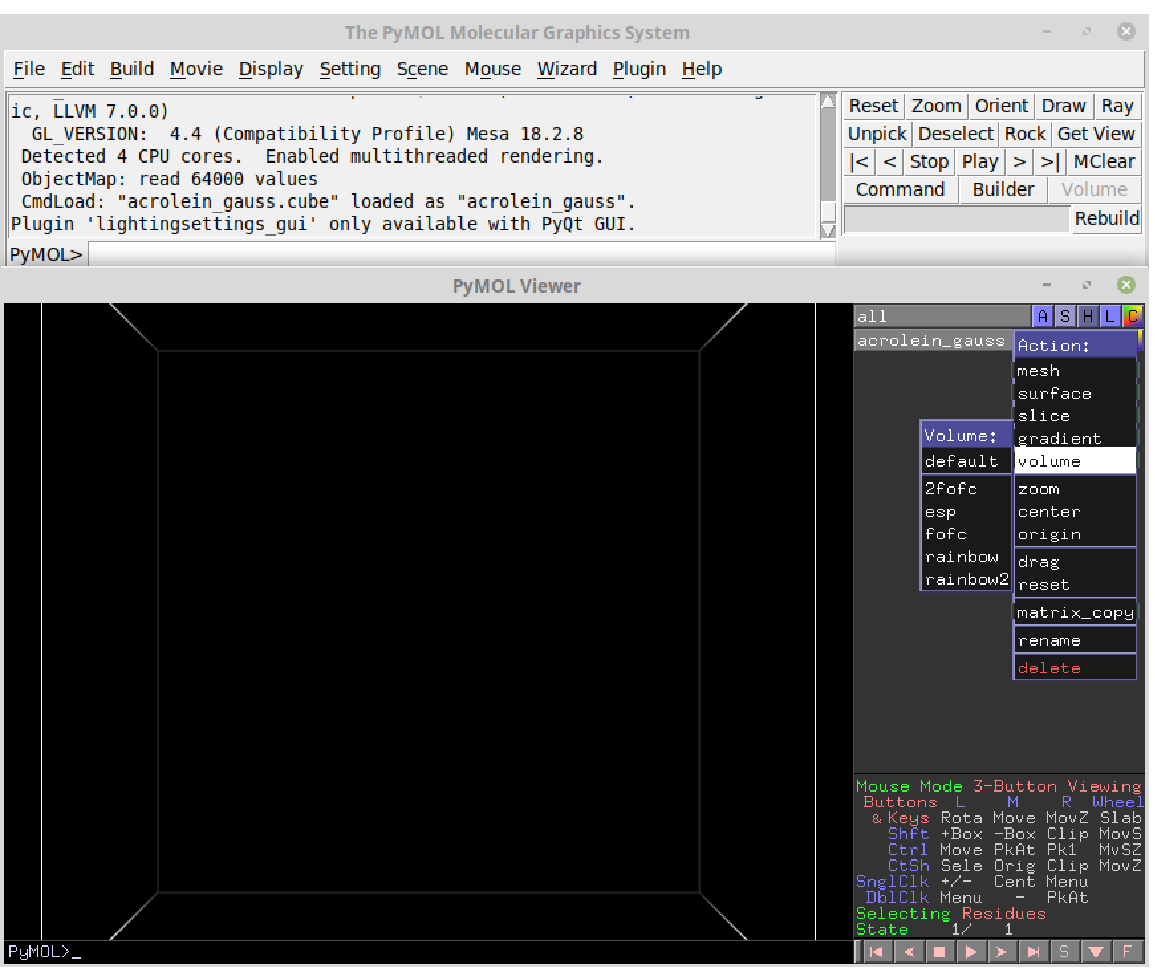
\includegraphics[width=5in]{figure1}
	\caption{Pymol software window showing the right side bar with volume rendering options.}
	\label{fig1}
\end{figure}

The Pymol window will open with the cube file loaded. To show the iso-surfaces go to the action options in the right side bar and click in \emph{"volume"} and \emph{"default"}, as showed in \autoref{fig1}. To save the image, write in the Pymol terminal emulator   \emph{"draw 800,600"} to render a 800X600 pixel images and \emph{"png acrolein\_gaus.png"} to save in png format, that is shown in \autoref{fig2}. This set of instructions can be followed to generate the images from volume rendering in Pymol in the next tutorial steps. 

\begin{figure}[H]
	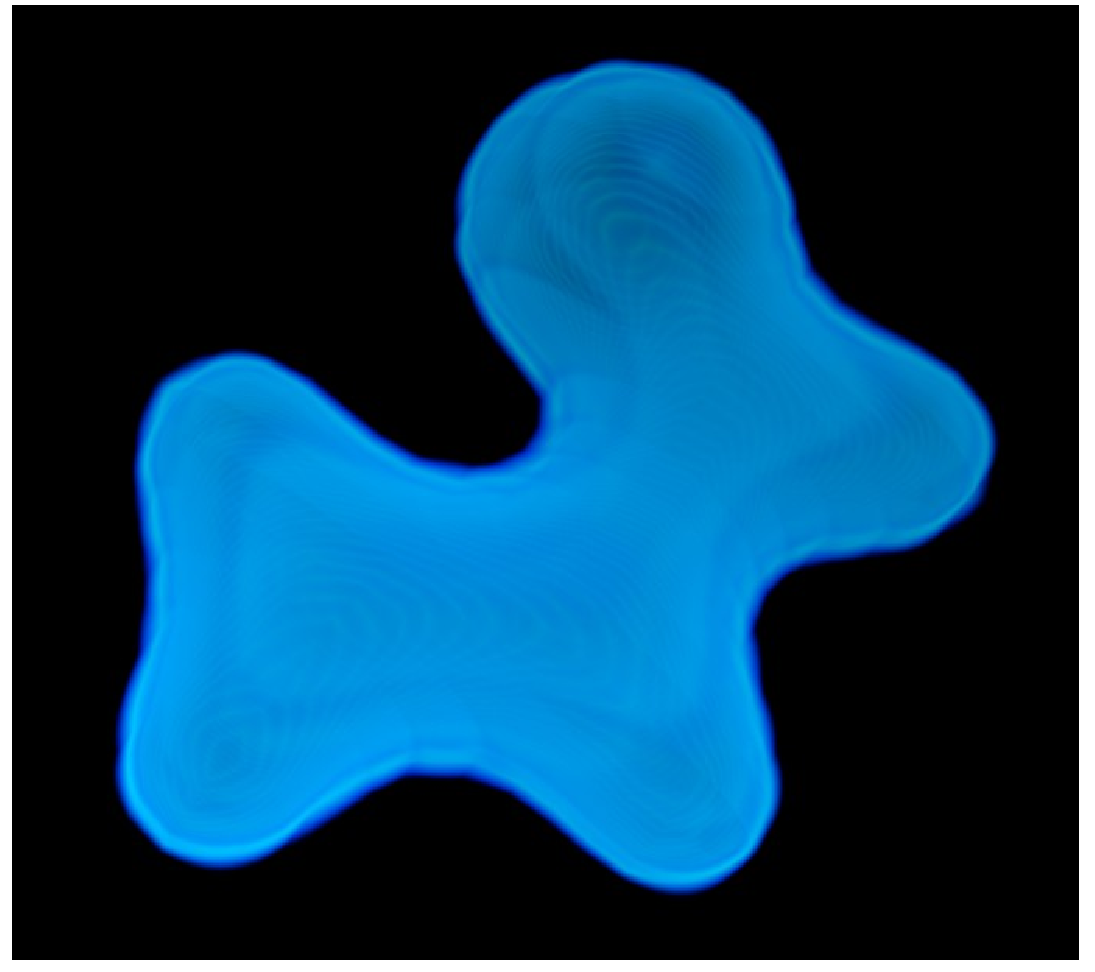
\includegraphics[width=4in]{figure2}
	\caption{Acrolein total electron density calculated by PRIMoRDiA and saved from Pymol }
	\label{fig2}
\end{figure} 

The generation of Molecular Orbitals 


\hspace*{-\leftmarginwidth}
\begin{minipage}{\fullwidth}
	\begin{commandshell}
		primordia -mo acrloein_gauss.fchk  40 gaussian
	\end{commandshell}
\end{minipage}


\subsection{Reactivity Descriptors Calculations}

\subsubsection{Global Reactivity Descriptors}

\subsubsection{Local Reactivity Descriptors: Volumetric}

\subsubsection{Local Reactivity Descriptors: Condensed}
 
\subsubsection{Band Reactivity Descriptor: Small Peptides}

\subsubsection{Band Reactivity Descriptors: Enzymatic Reaction}



\bibliographystyle{ieeetr}
\newpage
\bibliography{bibliography}




%\begin{leftbar}

%\end{leftbar}

\end{document}